\chapter{The SMBO Paradigm}\label{ch:smbo}

\section{The Bootstrapping Cycle}

This thesis will explore several algorithms that are classified as sequential model-based optimizers \cite{hutter_sequential_2011, hamadi_autonomous_2012, jones_efficient_1998, rasmussen_gaussian_2006}. %note: get more specific with those cites. should be a handful of specific papers presenting particular SMBO things
They differ in the space of model functions they explore, their assumptions regarding determinism, and their procedural relationship to the objective functions being optimized. % clarification: such as some algorithms selecting one sample point, others more.
Nonetheless, they can all be roughly summarized by a three-part loop,

\begin{enumerate} \label{smbo_loop}
\item the objective function is evaluated at some set of input points
\item a working model of the objective function (the ``predictor function'') is generated from the evaluated input-output pairs
\item new points are chosen to be evaluated by the objective function, so that the working model's utility in optimizing the objective function will be maximized.
\end{enumerate}

[note: should the above be in pseudocode? It would at least be nice to reference it like a figure.]

The loop is run until results are satisfactory, or the expected improvement from further iterations falls below a user-defined threshold. Because of the circular, bootstrapping nature of the algorithm, it is tempting to illustrate it with a triangle like we see on recycling bins, as shown in Figure \ref{fig:smbo_cycle}

\begin{figure}[h]
	\centering
	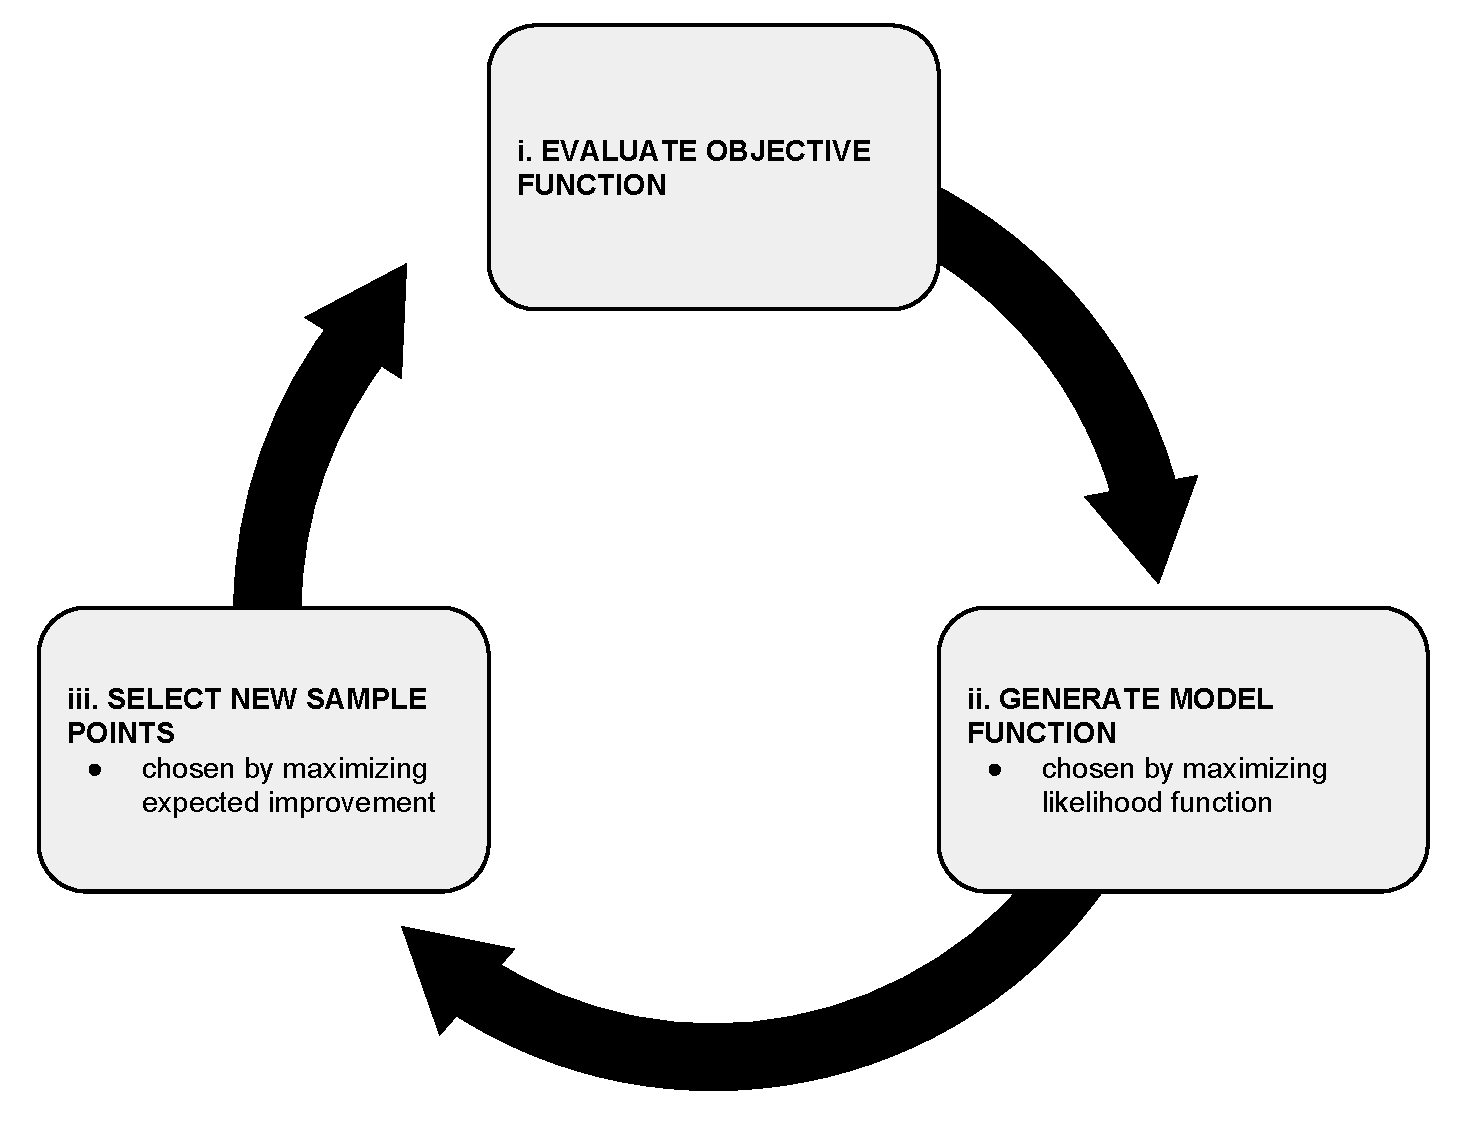
\includegraphics[width=0.5\textwidth]{EGO_cycle}
	\caption{the three iterated stages of the SMBO process}
	\label{fig:smbo_cycle}

\end{figure}

Tho company ProtoLife uses a similar illustration to Fig. \ref{fig:smbo_cycle} to describe their analytical product, which appears to be a powerful research application of SMBO \citep{protolife_pdt_2013}. The top node in the triangle is determined by each domain-specific application. Like ProtoLife, I am interested in trying several different model modules (the bottom-right node in the figure) to optimize different objective functions (the top-right node). A recent PhD dissertation on SMBO also included a nearly identical figure \cite{hutter_sequential_2011}; it is clear that the image above, and the tripartite view of SMBO it illustrates, is the most popular conceptualizing of sequential model-based optimization.

[Hutter aslo includes in his introduction an image of a predictor function w/ expected improvement overlayed, like in Jones, right here]

\section{Terms, Symbols}

I will quickly present a list of technical terms and symbols which will be useful in the presentation of this material.

The function which we wish to optimize is the \emph{objective function}. This term comes from statistics and regression---for some reason the name ``blackbox function'' is more popular in discussing general algorithm design than in rigorous definitions. This being model-based optimization, a central component will be the \emph{predictor} or \emph{model function}---that which is generated in each iteration of the loop illustrated in Fig \ref{fig:smbo_cycle}. I will refer to that loop as the \emph{SMBO loop} (or \emph{cycle}), which contains three nodes or modules. 

\emph{Sample points} are those points where we have evaluated the objective function--the points on which we base our model function. Throughout this thesis, I'll use several letters and symbols for specific concepts and indices. So that there is a definitive reference, I have listed them here (make this an official table/figure?).

\begin{description}
  \item[$n$]: the number of sample points
  \item[$k$]: the dimensionality of input space
  \item[$\X^{(i)}$]: the $i$th sample point (a $k$-vector)
  \item[$\X$]: the vector of sample points ($n$ $k$-vectors, an $n\times k$ matrix)
  \item[$y$]: the objective function
  \item[$\hat{y}$]: the predictor function
  \item[$\Y$]: the vector of evaluated outputs, i.e. $\Y_i=y(\X^{(i)})$
\end{description}

In the vocabulary of above, each stage in the SMBO loop can be defined as a mathematical function:
\begin{description}
	\item[\textbf{I}]: The objective function maps $k$-vectors from input-space to outputs.
	\item[\textbf{II}]: The model module maps the sample points to a model function.
	\item[\textbf{III}]: The sampling strategy is a function that takes as input a model function, and outputs the next $k$-vector(s) which should be evaluated by the objective.
\end{description}

Seeing each component as simply a function mapping a certain kind of input to a certain kind of output, combined with the circular relationship illustrated in Fig \ref{fig:smbo_cycle}, is what motivates me to describe the SMBO process as bootstrapping. From the perspective of node \textbf{I} in the cycle, the output of the objective function determines the next input of the objective function, which determines the next input, and do on. From the perspective of node \textbf{II}, each model induces the model that follows it.

\section{SMBO$_{III}: Maximum Improvement$}

The third step in the SMBO loop is perhaps the most characteristic---different SMBO algorithms use different model functions to accomplish the task in node \textbf{II}, and of course each implementation might attempt to optimize a unique objective function. The third step, however, has a standard solution that is relatively ubiquitous: maximizing a function of input space called \emph{expected improvement}. Expected improvement is one of those results from statistics that does a strikingly good job of quantifying a concept that seems, at first, to be too subtle to be straightforwardly quantified. It provides an answer to the question, ``how do I balance exploration with exploitation?"

There should be further discussion here. I think providing a fuller description of why the exploration/exploitation balance is hard to make, and why expected improvement accomplishes that, will be sufficient.

[Quote Donald Jones here about how neat expected improvement is].

\section{SMBO$_0$: The Initial Sample}

Obviously, it is impossible to construct a model of a blackbox function's response surface if you have not ever queried the blackbox, and a model based on one or very few sample points is not worth much. That is why any attempt at SMBO requires a strategy for picking initial sample points, which will induce an initial prediction model from which the SMBO loop can comfortably iterate. A common strategy (find sources on wikipedia) for selecting these points, and the only strategy I will consider in this thesis, is called a latin hypercube sample.

To construct an $n$-point latin hypercube in $k$ dimensions, first divide each dimension's domain into $n$ rows. This induces a grid, subdividing the original $k$-rectangular domain into $n^k$ sub-rectangles. A latin hypercube sample takes points from this domain under the constraint that no row in any one dimension contains two sample points.

That being said, the latin hypercube is one of those things that is more easily explained with pictures than words. [Put pictures here: is it cool to just life (and cite) the wikimedia commons pics from wikipedia?].

If you are a fan of sudoku, you have spent a lot of time thinking about latin hypercubes: the distribution of any one numeral across the game board matches a nine-sample two-dimensional latin hypercube. [Little picture demonstrating this, perhaps in a row with the wikipedia latin squares]


\section{Illustrative Examples}
Lets get some nice pictures in here




